%\documentclass[iop]{emulateapj}
%\documentclass[12pt, preprint]{emulateapj}
\documentclass[12pt, onecolumn]{emulateapj}

\usepackage{amsmath}
%\usepackage{bibtex}
%\bibliographystyle{unsrtnat}

\newcommand{\myemail}{aimalz@nyu.edu}
\newcommand{\textul}{\underline}

%\slugcomment{}

\shorttitle{Probabilistic inference of the Hubble parameter}
\shortauthors{Malz and Peters, et al.}

\begin{document}

\title{Probabilistic inference of the Hubble parameter}

\author{Alex Malz\altaffilmark{1}}
\author{Tina Peters\altaffilmark{2}}
\author{Humna Awan}
\author{Kara Ponder}
\author{Lluis Galbany}
\author{Anita Bahmanyar}
\altaffiltext{1}{Center for Cosmology and Particle Physics, Department of Physics,
  New York University, 4 Washington Pl., room 424, New York, NY 10003, USA}
 \altaffiltext{2}{Dunlap\dots}
\email{aimalz@nyu.edu}

\begin{abstract}
The BEAMS framework enables the use of probabilistic supernova classifications to estimate the Hubble parameter quantifying the relationship between distance and redshift over cosmic time.  This work extends BEAMS to replace high-confidence spectroscopic redshifts with probabilistic photometric redshifts, enabling inference of the Hubble parameter as a function of two probabilistic variables.  By combining posterior probabilities of supernova type and posterior probability distributions over host galaxy redshift, we infer a posterior probability distribution over the redshift-dependent Hubble parameter.  This work also produces a code that can be used for other regression problems in astrophysics that involve catalogs of two probabilistic variables.
\end{abstract}

\keywords{}

\section{Introduction}
\label{sec:intro}

\citet{kunz_bayesian_2007, kelly_flexible_2008}

\section{Methods}
\label{sec:meth}

This covers a complete sample, i.e. a catalog of all $N$ supernovae $ns$ in the universe, ever.  We'll add in the selection function later.

\vspace{1in}
\begin{figure}
\begin{center}
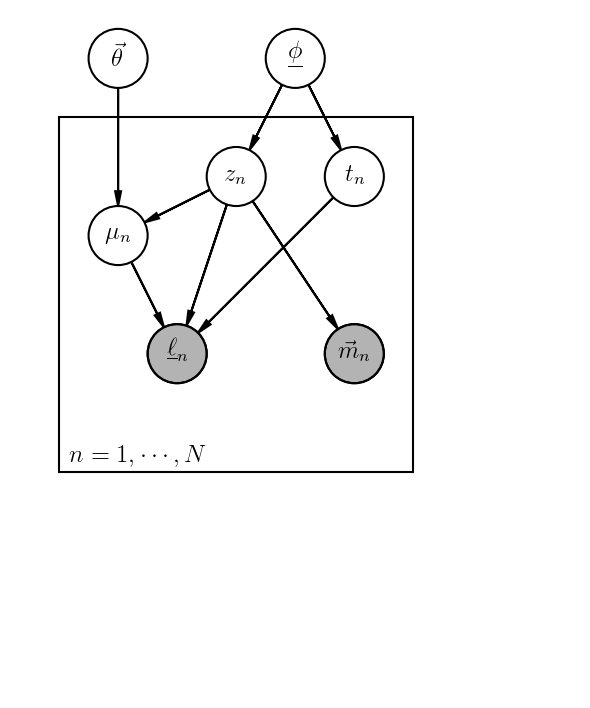
\includegraphics{Hubble-draft.png}
%\caption{}
\label{fig:pgm}
\end{center}
\end{figure}
\vspace{1in}

\begin{align}
p(\vec{\theta}, \textul{\Phi} | \{\textul{\ell}_{n}, \vec{f}_{n}\}_{N}) &\propto p(\vec{\theta}, \textul{\Phi})\ p(\{\textul{\ell}_{n}, \vec{f}_{n}\}_{N} | \vec{\theta}, \textul{\Phi})
\end{align}

\begin{align}
p(\{\textul{\ell}_{n}, \vec{f}_{n}\}_{N} | \vec{\theta}, \textul{\Phi}) &= \prod_{n}^{N}p(\textul{\ell}_{n}, \vec{f}_{n} | \vec{\theta}, \textul{\Phi})
\end{align}

\begin{align}
p(\textul{\ell}_{n}, \vec{f}_{n} | \vec{\theta}, \textul{\Phi}) &= \iiint p(\textul{\ell}_{n}, \vec{f}_{n} | \mu_{n}, z_{n}, T_{n})\ p(\mu_{n}, z_{n}, T_{n} | \vec{\theta}, \textul{\Phi})\ d\mu_{n}\ dz_{n}\ dT_{n}
\end{align}

\begin{align}
p(\textul{\ell}_{n}, \vec{f}_{n} | \mu_{n}, z_{n}, T_{n}) &= p(\textul{\ell}_{n}, \vec{f}_{n} | \mu_{n}, z_{n}, T_{n})\ \frac{p(\mu_{n}, z_{n}, T_{n} | \textul{\ell}_{n}, \vec{f}_{n}, \vec{\theta}^{*}, \textul{\Phi}^{*})}{p(\mu_{n}, z_{n}, T_{n} | \textul{\ell}_{n}, \vec{f}_{n}, \vec{\theta}^{*}, \textul{\Phi}^{*})}
\end{align}

\begin{align}
p(\mu_{n}, z_{n}, T_{n}|\textul{\ell}_{n}, \vec{f}_{n}, \vec{\theta}^{*}, \textul{\Phi}^{*}) &= \frac{p(\mu_{n}, z_{n}, T_{n} | \vec{\theta}^{*}, \textul{\Phi}^{*})\ p(\textul{\ell}_{n}, \vec{f}_{n} | \mu_{n}, z_{n}, T_{n}, \vec{\theta}^{*}, \textul{\Phi}^{*})}{p(\textul{\ell}_{n}, \vec{f}_{n} | \vec{\theta}^{*}, \textul{\Phi}^{*})}
\end{align}

\begin{align}
p(\textul{\ell}_{n}, \vec{f}_{n} | \mu_{n}, z_{n}, T_{n}, \vec{\theta}^{*}, \textul{\Phi}^{*}) &= p(\textul{\ell}_{n}, \vec{f}_{n} | \mu_{n}, z_{n}, T_{n})\ p(\textul{\ell}_{n}, \vec{f}_{n} | \vec{\theta}^{*}, \textul{\Phi}^{*})
\end{align}

\begin{align}
p(\textul{\ell}_{n}, \vec{f}_{n} | \mu_{n}, z_{n}, T_{n}) &= \frac{p(\mu_{n}, z_{n}, T_{n} | \textul{\ell}_{n}, \vec{f}_{n}, \vec{\theta}^{*}, \textul{\Phi}^{*})}{p(\mu_{n}, z_{n}, T_{n} | \vec{\theta}^{*}, \textul{\Phi}^{*})}
\end{align}

\begin{align}
p(\textul{\ell}_{n}, \vec{f}_{n} | \vec{\theta}, \textul{\Phi}) &= \iiint p(\mu_{n}, z_{n}, T_{n} | \textul{\ell}_{n}, \vec{f}_{n}, \vec{\theta}^{*}, \textul{\Phi}^{*})\ \frac{p(\mu_{n}, z_{n}, T_{n} | \vec{\theta}, \textul{\Phi})}{p(\mu_{n}, z_{n}, T_{n} | \vec{\theta}^{*}, \textul{\Phi}^{*})}\ d\mu_{n}\ dz_{n}\ dT_{n}
\end{align}

\begin{align}
p(\{\textul{\ell}_{n}, \vec{f}_{n}\}_{N} | \vec{\theta}, \textul{\Phi}) &= \prod_{n}^{N}\ \iiint p(\mu_{n}, z_{n}, T_{n} | \textul{\ell}_{n}, \vec{f}_{n}, \vec{\theta}^{*}, \textul{\Phi}^{*})\ \frac{p(\mu_{n}, z_{n}, T_{n} | \vec{\theta}, \textul{\Phi})}{p(\mu_{n}, z_{n}, T_{n} | \vec{\theta}^{*}, \textul{\Phi}^{*})}\ d\mu_{n}\ dz_{n}\ dT_{n}
\end{align}

\begin{align}
p(\vec{\theta}, \textul{\Phi} | \{\textul{\ell}_{n}, \vec{f}_{n}\}_{N}) &\propto p(\vec{\theta}, \textul{\Phi})\ \prod_{n}^{N}\ \iiint p(\mu_{n}, z_{n}, T_{n} | \textul{\ell}_{n}, \vec{f}_{n}, \vec{\theta}^{*}, \textul{\Phi}^{*})\ \frac{p(\mu_{n}, z_{n}, T_{n} | \vec{\theta}, \textul{\Phi})}{p(\mu_{n}, z_{n}, T_{n} | \vec{\theta}^{*}, \textul{\Phi}^{*})}\ d\mu_{n}\ dz_{n}\ dT_{n}
\end{align}

\section{Data}
\label{sec:data}

\begin{align}
T_{n}' &\sim D[\vec{r}(T_{n})]\\
z_{n}' &\sim \vec{\Phi}(T_{n})\\
\mu_{n}' &= \mu(z_{n}', \vec{\theta})
\end{align}

%\acknowledgments

%\appendix

\bibliography{references}

\end{document}